\begin{center}
    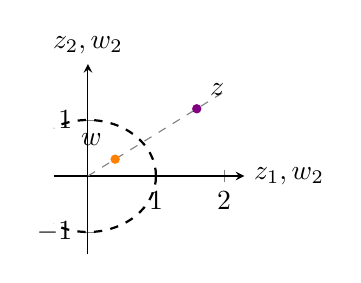
\begin{tikzpicture}
        [
            scale = 1.0,
            >=latex
        ]
        \begin{axis}[
            xmin=-0.5,
            xmax=2.3,
            ymin=-1.4,
            ymax=2,
            width=4cm,
            height=4cm,
            axis x line=middle, 
            axis y line=middle, 
            xtick={0, 1, 2},
            xticklabels={$0$, $1$, $2$},
            ytick={-1, 0, 1},
            x label style={anchor=west},
            xlabel={$\cvt{z_1}, \cor{w_2}$}, 
            y label style={anchor=south},
            ylabel={$\cvt{z_2}, \cor{w_2}$}
        ]
        
        % Cerchio unitario di riferimento
        \draw[black, thick, dashed] (axis cs:0,0) circle [radius=1];
        
        % Retta d'azione
        \addplot[gray, dashed, thin, domain=0:2] {0.75*x};
        
        % Punto z (|z| = 2)
        \node[circle, fill=violet, inner sep=1.2pt, label={above right:$z$}] at (axis cs:1.6, 1.2) {};
        
        % Punto w (immagine di z, |w| = 0.5)
        \node[circle, fill=orange, inner sep=1.2pt, label={above left:$w$}] at (axis cs:0.4, 0.3) {};

        \end{axis}
    \end{tikzpicture}
\end{center}